%% start of file `template.tex'.
%% Copyright 2006-2015 Xavier Danaux (xdanaux@gmail.com).
%
% Adapted to be an Rmarkdown template by Mitchell O'Hara-Wild
% 8 February 2019
%
% This work may be distributed and/or modified under the
% conditions of the LaTeX Project Public License version 1.3c,
% available at http://www.latex-project.org/lppl/.


\documentclass[11pt,a4paper,]{moderncv}

% moderncv themes
\moderncvstyle{casual}                             % style options are 'casual' (default), 'classic', 'banking', 'oldstyle' and 'fancy'

\definecolor{color0}{rgb}{0,0,0}% black
\definecolor{color1}{HTML}{414141}% custom
\definecolor{color2}{rgb}{0.45,0.45,0.45}% dark grey

\usepackage[scaled=0.86]{DejaVuSansMono}

\providecommand{\tightlist}{%
	\setlength{\itemsep}{0pt}\setlength{\parskip}{0pt}}
\def\donothing#1{#1}
\def\emaillink#1{#1}

%\nopagenumbers{}                                  % uncomment to suppress automatic page numbering for CVs longer than one page

% character encoding
%\usepackage[utf8]{inputenc}                       % if you are not using xelatex ou lualatex, replace by the encoding you are using
%\usepackage{CJKutf8}                              % if you need to use CJK to typeset your resume in Chinese, Japanese or Korean

% adjust the page margins
\usepackage[scale=0.75,footskip=60pt]{geometry}
%\setlength{\hintscolumnwidth}{3cm}                % if you want to change the width of the column with the dates
%\setlength{\makecvheadnamewidth}{10cm}            % for the 'classic' style, if you want to force the width allocated to your name and avoid line breaks. be careful though, the length is normally calculated to avoid any overlap with your personal info; use this at your own typographical risks...


\usepackage{fancyhdr}
\pagestyle{fancy}
\fancyhf{}
\fancyhead[R]{\thepage}

% personal data
\name{Sarah E}{Schwartz}
\title{Research Assistant Professor}
\address{Utah State University}{}{}
\phone[mobile]{(435) 797 - 0169} % Phone number
\email{\donothing{\href{mailto:Sarah.Schwartz@usu.edu}{\nolinkurl{Sarah.Schwartz@usu.edu}}}}
\homepage{www.SarahSchwartzStats.com} % Personal website
\social[linkedin]{SarBearSchwartz}
\social[twitter]{USU\_StatStudio}
\social[github]{SarBearSchwartz}
% \extrainfo{additional information}                 % optional, remove / comment the line if not wanted



\quote{I am a statistician with a passion for facilitating research that
is appropriate, transparent, and reproducible.}

% Pandoc CSL macros
\newlength{\cslhangindent}
\setlength{\cslhangindent}{1.5em}
\newlength{\csllabelwidth}
\setlength{\csllabelwidth}{3em}
\newenvironment{CSLReferences}[3] % #1 hanging-ident, #2 entry spacing
 {% don't indent paragraphs
  \setlength{\parindent}{0pt}
  % turn on hanging indent if param 1 is 1
  \ifodd #1 \everypar{\setlength{\hangindent}{\cslhangindent}}\ignorespaces\fi
  % set entry spacing
  \ifnum #2 > 0
  \setlength{\parskip}{#2\baselineskip}
  \fi
 }%
 {}
\usepackage{calc}
\newcommand{\CSLBlock}[1]{#1\hfill\break}
\newcommand{\CSLLeftMargin}[1]{\parbox[t]{\csllabelwidth}{#1}}
\newcommand{\CSLRightInline}[1]{\parbox[t]{\linewidth - \csllabelwidth}{#1}}
\newcommand{\CSLIndent}[1]{\hspace{\cslhangindent}#1}

%----------------------------------------------------------------------------------
%            content
%----------------------------------------------------------------------------------
\begin{document}
%\begin{CJK*}{UTF8}{gbsn}                          % to typeset your resume in Chinese using CJK
%-----       resume       ---------------------------------------------------------
\makecvtitle



\hypertarget{academic-appointment}{%
\section{Academic Appointment}\label{academic-appointment}}

\nopagebreak
    \cventry{2015-present}{Assistant Research Professor}{Psychology Department, College of Education and Human Services}{Utah State University}{}{\begin{itemize}%
\item Director, The Statistical Consulting Studio%
\item Instructor, graduate student quantitatice methods and statistics courses%
\end{itemize}}
    \cventry{2013-2015}{Statistician}{Office of Research Services, College of Education and Human Services}{Utah State University}{}{\begin{itemize}%
\item Acting Director, Office of Methodological and Data Sciences%
\item Instructor, graduate student quantitatice methods and statistics courses%
\end{itemize}}
    \cventry{2005-2013}{Statistician and Data Manager}{Center for Epidemiology}{Utah State University}{}{\begin{itemize}%
\item Managed databases, clean data, and prepare custom datasets%
\item Performed statistical analyses and prepared publications, posters, presentations,
and grant submissions%
\item Worked under three main grants and many co-investigators: University of Utah,
  BYU, Duke, John Hopkins, University of Maryland, ect.%
\end{itemize}}
    \cventry{2012}{Data Manager}{Kenoi Genetics Lab}{Brigham Young University}{}{\begin{itemize}%
\item Managed databases and prepare custom datasets%
\end{itemize}}
    \cventry{2006-2008}{Adjunct Lecturer}{Mathematics and Statistics Department}{Utah State University}{}{\begin{itemize}%
\item Traditional, evening, and distance courses%
\end{itemize}}
    \cventry{2000-2004}{High School Teacher, Math and Science}{Mathematics and Statistics Department}{Utah State University}{}{\begin{itemize}%
\item Sky View High School, Smithfield, Utah%
\item Logan River Academy, Logan, Utah%
\end{itemize}}

\vspace{5 mm}

\hypertarget{certificates}{%
\section{Certificates}\label{certificates}}

\nopagebreak
    \cventry{2001-2009}{Teaching License}{Secondary Education}{State of Utah}{}{\begin{itemize}%
\item Endorsements: mathematics level 4 and chemistry%
\end{itemize}}

\clearpage

\hypertarget{education}{%
\section{Education}\label{education}}

\nopagebreak
    \cventry{2013-2017}{PhD: Mathetatics, Specialization in Statistics}{Utah State University}{Logan, Utah, USA}{}{\begin{itemize}%
\item TA: Lecturer and grader%
\item RA: Simulation programmer, Cytel Software Inc.%
\end{itemize}}
    \cventry{2004-2006}{MS: Statistics}{Utah State University}{Logan, Utah, USA}{}{\begin{itemize}%
\item Mentor: Dr. Chris Corcoran%
\item TA: Lecturer and grader%
\item RA: Statistician, Center for Epidemiology Studies%
\end{itemize}}
    \cventry{1998-2000}{BS: Math and Chem Secondary Education}{Utah State University}{Logan, Utah, USA}{}{\begin{itemize}%
\item Student Teaching: Sky View High School, Smithfield, Utah%
\end{itemize}}

\vspace{5 mm}

\hypertarget{awards-and-honors}{%
\section{Awards and Honors}\label{awards-and-honors}}

\nopagebreak
    \cventry{2015}{Department Academic Excellence Award}{Mathematics and Statistics Department}{Utah State University}{}{\empty}
    \cventry{2014}{Department Industrious Graduate Student Award}{Mathematics and Statistics Department}{Utah State University}{}{\empty}
    \cventry{2005}{Department Graduate Student Teacher of the Year Award}{Mathematics and Statistics Department}{Utah State University}{}{\empty}

\clearpage

\hypertarget{grants-funded}{%
\section{Grants: Funded}\label{grants-funded}}

\nopagebreak
    \cventry{Sept. 2019 - Feb. 2022}{National Science Foundation: Division Of Research On Learning}{Research on the Development of An Assessment to Measure Kindergarten Children's Abilities to Reason Computationally With Mathematical Problem-Solving Skills}{Utah State University}{}{\begin{itemize}%
\item Program: STEM + Computing (STEM+C) Part%
\item PI: Jody Clarke Midura%
\item Co-PI: Victor Raymond Lee, Jessica Shumway%
\item DUNS ID: 072983455%
\item Amount: \$1,120,807%
\end{itemize}}
    \cventry{July 2008 - June 2011}{National Institute of Health: National Institute on Aging}{R01 Grant: Lifespan Stressors and Alzheimer’s Disease: The Cache County Study.}{Utah State University}{}{\begin{itemize}%
\item Pis: Dr. Maria Norton%
\item Co-PI: Dr. Joann Tschanz%
\item Roll: data management and analysis%
\item Amount:  \$970,549 (original)%
\end{itemize}}
    \cventry{Sept. 2002 – Sept. 2013}{National Institute of Health: National Institute on Aging}{R01 Grant: Progression of Dementia, A Population Study.}{Utah State University}{}{\begin{itemize}%
\item PIs: Dr. Joann Tschanz and  Dr. Constantine G. Lyketsos%
\item Roll: data management and analysis%
\item DUNS ID: 072983455 (original)%
\item Amount: \$2,787,792 (original)%
\item Extended multiple times%
\end{itemize}}
    \cventry{Sept 2000 - Sept 2005}{National Institute of Health: National Institute on Aging}{R01 Grant: Cache County Family-based Cohort Study on Aging.}{Utah State University}{}{\begin{itemize}%
\item Pis: Drs John Breitner, Kathy Welch-Bohmer%
\item Roll: data management and analysis%
\item Amount \$1,999,400(original)%
\item Extended multiple times%
\end{itemize}}

\hypertarget{grants-submitted-or-revising}{%
\section{Grants: Submitted or
Revising}\label{grants-submitted-or-revising}}

\nopagebreak
    \cventry{Oct 2021}{National Science Foundation: Graduate Research Fellowships Program (GRFP)}{Fellowship:Risk Factors that Predict Cognitive Resilience in Older Adults at High Risk for Alzheimer’s Disease}{Utah State University}{}{\begin{itemize}%
\item PI: Hector Gonzalez%
\item Submitted%
\end{itemize}}
    \cventry{May 2021}{ACL National Institute on Disability, Independent Living, and Rehabilitation Research: Disability and Rehabilitation Research Projects and Centers Program (DPCP21000189)}{The Clubhouse Model as an Intervention to Address Social Isolation and Loneliness Among People with Severe Mental Illness}{Utah State University}{}{\begin{itemize}%
\item PI: Dr. Brian Phillips%
\item co-PIs: DRs Sarah E Schwartz, Allison Fleming, Colleen McKay%
\item Amount: \$2,715,870 (5 years)%
\item Score: 82/100 (73-86)%
\item Currently revising%
\end{itemize}}
    \cventry{November 2020}{National Institute of Health:  Global Brain and Nervous System Disorders Research Across the Lifespan (PAR-18-835)}{R21 Grant: Buenas Bases: An Early Childhood Development Intervention for Children of Ecuadorian Adolescent Mothers}{Utah State University}{}{\begin{itemize}%
\item PIs: Drs. Edwardo Ortiz, Lisa Boyce%
\item coPIs: Drs. Ryan Seedall, Eric Reither, Sarah E Schwartz, Spencer Bradshaw, Marcela Santos, Sonia Rodrigues-Jaramillo, Patricial Ordonez, Jill Luto%
\item Amount: \$3,168,557%
\item Application Number: 1 R01 HD106272-01%
\item Impact Score:50     Percentile:45%
\item Currently resubmitting%
\end{itemize}}
    \cventry{Febuary 2020}{National Institute of Health:  National Institute of Child Health and Human Development (PA-18-482)}{R21 Grant: The Effect of Background Noise on Reading Performance in Children with ASD}{Utah State University}{}{\begin{itemize}%
\item Amount \$2,445,008 (4 years)%
\item PI: Dr Maryellen McClain Verdose%
\item co-PI: Drs Sarah Yoho Leopold, Sarah E Schwartz%
\item Amount \$385,648 (2 years)%
\item Application Number: 1 R21 HD103992-01%
\item Currently resubmitting%
\end{itemize}}
    \cventry{October 2019, November 2020}{National Institute of Health: National Institute of Aging (PA-20-185)}{R01 Grant: Response Inhibition in Reactive Balance Control}{Utah State University}{}{\begin{itemize}%
\item PI: Dr Dave Bolton%
\item co-PIs: Drs JoAnn Tschanz, Chris Warren, Sarah E Schwartz%
\item Amount \$2,445,008 (4 years)%
\item NIH Appl. ID: 10030557%
\item Currently resubmitting%
\end{itemize}}

\clearpage

\hypertarget{publications}{%
\section{Publications}\label{publications}}

\begin{center}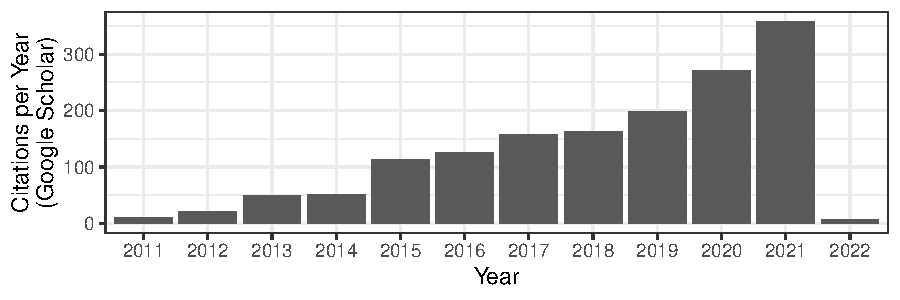
\includegraphics{SchwartzSarah_CV_short_files/figure-latex/unnamed-chunk-1-1} \end{center}

\hypertarget{working-papers-under-revision-or-review}{%
\subsection{\texorpdfstring{\textbf{Working Papers under Revision or
Review}}{Working Papers under Revision or Review}}\label{working-papers-under-revision-or-review}}

\hypertarget{refs_journalspress}{}

\vspace{7mm}

\hypertarget{refereed-journal-papers---2022}{%
\subsection{\texorpdfstring{\textbf{Refereed Journal Papers -
2022}}{Refereed Journal Papers - 2022}}\label{refereed-journal-papers---2022}}

\hypertarget{refs_journals2022}{}

\hypertarget{refereed-journal-papers---2021}{%
\subsection{\texorpdfstring{\textbf{Refereed Journal Papers -
2021}}{Refereed Journal Papers - 2021}}\label{refereed-journal-papers---2021}}

\hypertarget{refs_journals2021}{}

\vspace{7mm}

\hypertarget{refereed-journal-papers---2020}{%
\subsection{\texorpdfstring{\textbf{Refereed Journal Papers -
2020}}{Refereed Journal Papers - 2020}}\label{refereed-journal-papers---2020}}

\hypertarget{refs_journals2020}{}

\vspace{7mm}

\hypertarget{refereed-journal-papers---2019}{%
\subsection{\texorpdfstring{\textbf{Refereed Journal Papers -
2019}}{Refereed Journal Papers - 2019}}\label{refereed-journal-papers---2019}}

\hypertarget{refs_journals2019}{}

\vspace{7mm}

\hypertarget{refereed-journal-papers---2018}{%
\subsection{\texorpdfstring{\textbf{Refereed Journal Papers -
2018}}{Refereed Journal Papers - 2018}}\label{refereed-journal-papers---2018}}

\hypertarget{refs_journals2018}{}

\vspace{7mm}

\hypertarget{refereed-journal-papers---2017-and-prior}{%
\subsection{\texorpdfstring{\textbf{Refereed Journal Papers - 2017 and
Prior}}{Refereed Journal Papers - 2017 and Prior}}\label{refereed-journal-papers---2017-and-prior}}

\hypertarget{refs_journals2017}{}

\clearpage

\hypertarget{papers-in-refereed-conference-proceedings}{%
\subsection{\texorpdfstring{\textbf{Papers in Refereed Conference
Proceedings}}{Papers in Refereed Conference Proceedings}}\label{papers-in-refereed-conference-proceedings}}

\hypertarget{refs_proceedings}{}

\vspace{7mm}

\hypertarget{conference-presentations-coauthored}{%
\subsection{\texorpdfstring{\textbf{Conference Presentations
Coauthored}}{Conference Presentations Coauthored}}\label{conference-presentations-coauthored}}

\hypertarget{refs_confco}{}

\vspace{7mm}

\hypertarget{work-not-peer-reviewed}{%
\subsection{\texorpdfstring{\textbf{Work Not Peer
Reviewed}}{Work Not Peer Reviewed}}\label{work-not-peer-reviewed}}

\hypertarget{refs_notpeer}{}

\vspace{7mm}

\hypertarget{disertation}{%
\subsection{\texorpdfstring{\textbf{Disertation}}{Disertation}}\label{disertation}}

\hypertarget{refs_student}{}

\vspace{7mm}

\hypertarget{online-ebook}{%
\subsection{\texorpdfstring{\textbf{Online
eBook}}{Online eBook}}\label{online-ebook}}

\hypertarget{refs_ebook}{}

\hypertarget{notes}{%
\section{Notes}\label{notes}}

\begin{itemize}
\tightlist
\item
  This CV is reproducible; all the source code behind this CV is
  available on \href{https://github.com/sarbearschwartz/jy_CV}{this
  GitHub repo}.
\end{itemize}


\end{document}

%\clearpage\end{CJK*}                              % if you are typesetting your resume in Chinese using CJK; the \clearpage is required for fancyhdr to work correctly with CJK, though it kills the page numbering by making \lastpage undefined
\end{document}


%% end of file `template.tex'.
